%\documentclass[referee]{aa} % for a referee version
%\documentclass[onecolumn]{aa} % for a paper on 1 column  
%\documentclass[longauth]{aa} % for the long lists of affiliations 
%\documentclass[letter]{aa} % for the letters 
\documentclass{aa}

\usepackage{txfonts}
\usepackage{natbib}

\usepackage{graphicx}

\usepackage{color}
\usepackage{hyperref}
\hypersetup{colorlinks=true,allcolors=[rgb]{0,0,0.8}}


\usepackage{showyourwork}

% the three lines suppress the hyperref 'link empty' warnings
% explanation at: https://tex.stackexchange.com/questions/345764/journal-class-shows-package-hyperref-warning-suppressing-link-with-empty-targe
%\makeatletter
%\renewcommand*\aa@pageof{, page \thepage{} of \pageref*{LastPage}}
%\makeatother

% text highlighting
%\usepackage{soul}
%\sethlcolor{yellow}


\newcommand{\asas}{ASASSN-21qj}
\newcommand{\ktwo}{\textit{K2}}
\newcommand{\kms}{km~s$^{-1}$\xspace}
\newcommand{\ms}{m~s$^{-1}$}
\newcommand{\gcc}{g~cm$^{-3}$}
\newcommand{\masyr}{mas~yr$^{-1}$}
\newcommand{\err}{\textit{$\pm$}}
\newcommand{\teff}{$T_\mathrm{eff}$}
\newcommand{\msun}{$M_\odot$}
\newcommand{\rsun}{$R_\odot$}
\newcommand{\lsun}{$L_\odot$}
\newcommand{\rhosun}{$\rho_\odot$}
\newcommand{\mstar}{$M_*$}
\newcommand{\rstar}{$R_*$}
\newcommand{\lstar}{$L_*$}
\newcommand{\rearth}{$R_\oplus$}
\newcommand{\vrad}{$v_{R}$}
\newcommand{\pmra}{$\mu_{\alpha}$}
\newcommand{\pmdec}{$\mu_{\delta}$}

\newcommand{\rhostar}{$\rho_*$}
\newcommand{\mjup}{$M_\mathrm{Jup}$}
\newcommand{\galex}{\textit{GALEX}}
\newcommand{\gaia}{\textit{Gaia}}
\newcommand{\kepler}{\textit{Kepler}}
\newcommand{\spitzer}{\textit{Spitzer}}
\newcommand{\ktwosc}{\textsc{k2sc}}
\newcommand{\ktwosff}{\textsc{k2sff}}
\newcommand{\hipparcos}{\textit{Hipparcos}}
\newcommand{\tess}{\textit{TESS}}
\newcommand{\emcee}{\textsc{emcee}}
\newcommand{\python}{\textsc{python}}


\begin{document} 
\authorrunning{Kenworthy et al.}
\titlerunning{Planetary collision afterglow}
   \title{The eclipse of ASASSN-21qj: A planetary collision afterglow\\ and transit of the resultant debris cloud}

   \author{Matthew A. Kenworthy
          \inst{1}
          \and
          Arttu Sainio
          \inst{1}
          \and
          Eric E. Mamajek
          \inst{1}
          \and
          Joseph Masiero
          \inst{1}
          \and
          Amy Mainzer
          \inst{1}
          \and
          Joseph (Davy) Kirkpatrick
          \inst{1}
          \and 
          Richelle F. van Capelleveen
          \inst{1}
          \and
          Grant M. Kennedy
                    \inst{1}
          \and
          Ludmila Carone
                    \inst{1}
          \and
          NEOWISE authorship list
                    \inst{1}
          \and
          AAVSO observers
                    \inst{1}
          \and
          St\'{e}phane Charbonnel
                    \inst{1}
          \and
        Olivier Garde
                  \inst{1}
        \and
        Pascal Le D\^{u}
                  \inst{1}
        \and
        Lionel Mulato
                  \inst{1}
        \and
        Thomas Petit
                  \inst{1}
          }

   \institute{Leiden Observatory, University of Leiden,
   PO Box 9513, 2300 RA Leiden, The Netherlands\\
   \email{kenworthy@strw.leidenuniv.nl}
%         \and
%             Arttu's address\\
%    \and
%    JPL
%    \and
%    Caltech/IPAC, 1200 E California Blvd, Mail Code 100-22, Pasadena, CA 91125, USA
%    \and
%    NEOWISE
%    \and
%    AAVSO people
%    \and
%    Space Research Institute, Austrian Academy of Sciences, Schmiedlstrasse 6, A-8042 Graz, Austria
}
   \date{Received XXXX; accepted XXXX}

% \abstract{}{}{}{}{} 
% 5 {} token are mandatory
 
  \abstract
  % context heading (optional)
  % {} leave it empty if necessary  
   {Towards the end of the planet forming process around stars, collisions between large planetessimals results in a collisional casade that results in sub-micron sized dust that is visible as a debris disk. 
   %
   The occurrence rate and brightness of debris disks decreases with increasing age, but there are several stars with infrared excesses that show significant quasi-stochastic variability in the infrared.
   %
   This is interpreted as dust generated from collisions close to the star that is subsequently heated by the stellar flux to become visible at infrared wavelengths.}
  % aims heading (mandatory)
   {A deep optical eclipse seen towards the young star \asas{} shows the transit of a large extended cloud of sub-micron sized dust, and an archival search of NEOWISE showed a significant infrared brightening some 900 days before the start of the eclipse.
   %
   We develop several hypotheses for this infrared brightening and optical eclipse and discuss which is the most consistent with our observations.
   show that the most likely explanation is a collision between two Neptune mass planets out at a distance o}
  % methods heading (mandatory)
   {We use multiband photometric monitoring of the eclipse for multiple telescopes to constrain the mass and transverse velocity of the cloud, and TESS photometry to identify the star as a rapid rotator consistent with a young ($\sim$ 100~Myr) stellar system.}
  % results heading (mandatory)
   {Our most likely hypothesis is that there was a collision between two Neptune sized exoplanets, resulting in a expanding cloud of condensing silicate vapour and rocky planetessimal debris, expanding and being sheared by Keplerian motion along the orbital track of the remnant that subsequently transited our line of sight.
   %
   The high colour temperature of the dust ($T=1000$\,K) implies that the expanding optically thick cloud of dust is heated by a $T\sim 2000$\,K collision remnant.
   %
   This appears to be the first detection of the afterglow of the collision remnant and the subsequent transit of the debris cloud in front of the star.
   %
   %We estimate that dust has a lower mass limit of \hl{XXXX} Earths.
   }
  % conclusions heading (optional), leave it empty if necessary 
   {}

   \keywords{circumstellar matter -- infrared: planetary systems -- planets and satellites: dynamical evolution and stability - stars: individual (ASASSN-21qj)}

   \maketitle
%
%-------------------------------------------------------------------

   \section{Introduction}

Debris disks are formed at the end of the planet formation epoch around main sequence stars, when the majority of the circumstellar gas has been removed through accretion, photoevaporation or stellar winds.
%
Debris disks are formed at the end of the planet formation epoch around main sequence stars, when the majority of the circumstellar gas has been removed through accretion, photoevaporation or stellar winds.Debris disks are formed at the end of the planet formation epoch around main sequence stars, when the majority of the circumstellar gas has been removed through accretion, photoevaporation or stellar winds.Debris disks are formed at the end of the planet formation epoch around main sequence stars, when the majority of the circumstellar gas has been removed through accretion, photoevaporation or stellar winds.Debris disks are formed at the end of the planet formation epoch around main sequence stars, when the majority of the circumstellar gas has been removed through accretion, photoevaporation or stellar winds.Debris disks are formed at the end of the planet formation epoch around main sequence stars, when the majority of the circumstellar gas has been removed through accretion, photoevaporation or stellar winds.Debris disks are formed at the end of the planet formation epoch around main sequence stars, when the majority of the circumstellar gas has been removed through accretion, photoevaporation or stellar winds.Debris disks are formed at the end of the planet formation epoch around main sequence stars, when the majority of the circumstellar gas has been removed through accretion, photoevaporation or stellar winds.Debris disks are formed at the end of the planet formation epoch around main sequence stars, when the majority of the circumstellar gas has been removed through accretion, photoevaporation or stellar winds.Debris disks are formed at the end of the planet formation epoch around main sequence stars, when the majority of the circumstellar gas has been removed through accretion, photoevaporation or stellar winds.

%\begin{figure*}
 %   \centering
 %   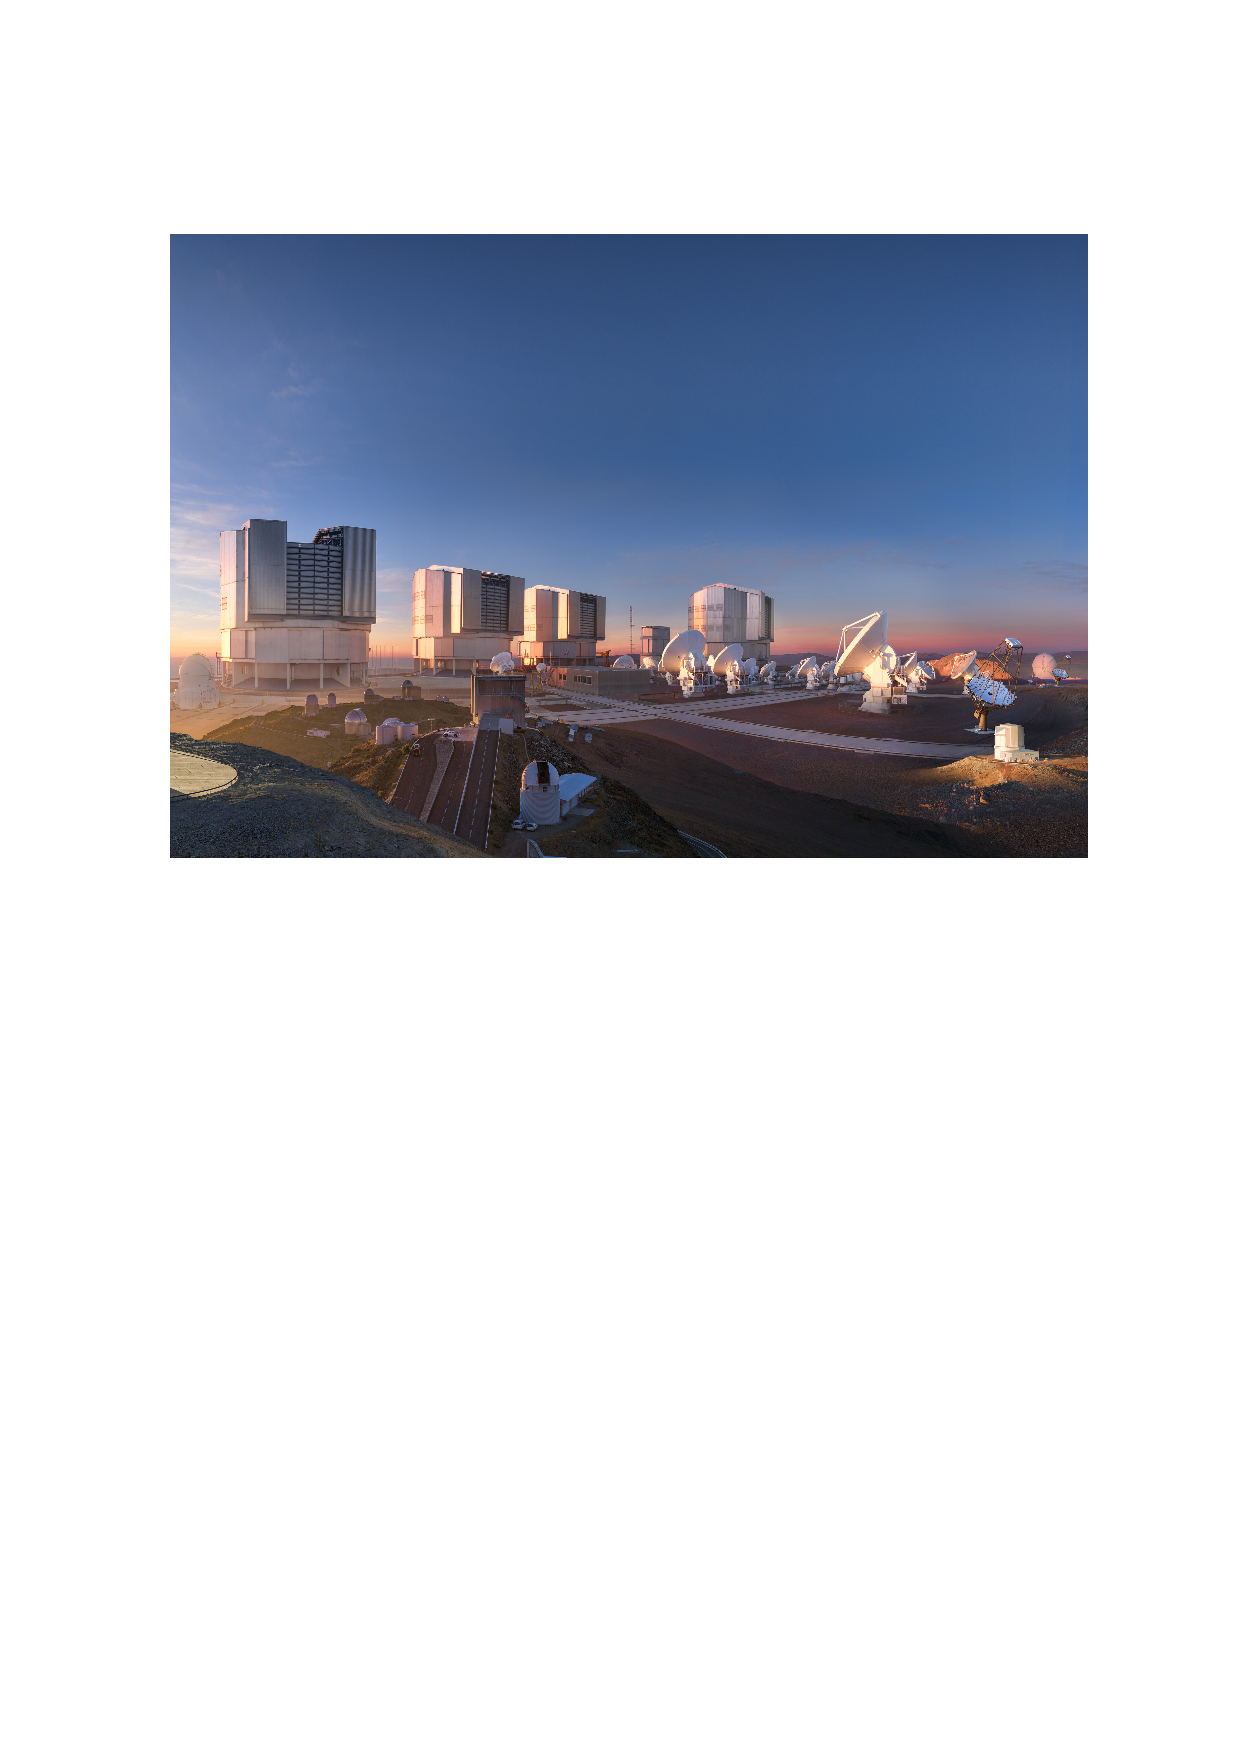
\includegraphics[width=1\textwidth]{figures/blueing.pdf}
 %   \caption{Blueing of the $B-V$ colour during dimming.
 %   %
 %   Points show AAVSO data, and lines show models.
 %   %
 %   The dashed line is a line of $A_\lambda/A_V$ for the value shown in the %legend in each panel, and the solid line is a model that includes an underlying scattered light component with $s=7.5$\% of the stellar flux.}
  %  \label{fig:blueing}
%    \script{blueing.py}
%\end{figure*}


\begin{acknowledgements}

This research has used the SIMBAD database, operated at CDS, Strasbourg, France \citep{wenger2000}.
%
This work has used data from the European Space Agency (ESA) mission {\it Gaia} (\url{https://www.cosmos.esa.int/gaia}), processed by the {\it Gaia} Data Processing and Analysis Consortium (DPAC, \url{https://www.cosmos.esa.int/web/gaia/dpac/consortium}).
%
To achieve the scientific results presented in this article we made use of the \emph{Python} programming language\footnote{Python Software Foundation, \url{https://www.python.org/}}, especially the \emph{SciPy} \citep{virtanen2020}, \emph{NumPy} \citep{numpy}, \emph{Matplotlib} \citep{Matplotlib}, \emph{emcee} \citep{foreman-mackey2013}, and \emph{astropy} \citep{astropy_1,astropy_2} packages.
%
This publication makes use of VOSA, developed under the Spanish Virtual Observatory project supported by the Spanish MINECO through grant AyA2017-84089.
%
This publication makes use of VOSA, developed under the Spanish Virtual Observatory\footnote{\url{https://svo.cab.inta-csic.es}} project funded by MCIN/AEI/10.13039/501100011033/ through grant PID2020-112949GB-I00.
%
VOSA has been partially updated by using funding from the European Union's Horizon 2020 Research and Innovation Programme, under Grant Agreement 776403 (EXOPLANETS-A). 
%
\end{acknowledgements}

\bibliographystyle{aa}
\bibliography{bib}

\end{document}
